\section{Study of Transfer learning methods}
\subsection{Downstream Task}
The performance of pre-trained T5 model is verified on following NLP benchmarks. \textbf{In this report, the findings are reported only on GLUE tasks considering space constraints. For full complete set of results, please refer the original paper. }
\begin{enumerate}
    \item GLUE and Super GLUE task: It comprises of diverse set of tasks to test the natural language understanding abilities including 
    \begin{enumerate}
        \item Sentence acceptability 
        \item Sentence analysis
        \item Sentence similarity
        \item Natural language inference
        \item Co-reference resolution
        \item sentence completion
        \item Word sense disambiguation
        \item Question answering
    \end{enumerate}
    \item Text summarization on CNN/Daily Mail
    \item Question answering on SQuAD dataset
    \item English to German, English to French, English to Romanian Machine translation 
\end{enumerate}

\subsection{Architecture}
The main differences in the architecture design in transfer learning setting arise from the type of masking used in the model. Masking is used to impose constraints on which tokens in the sequence the input token can attend to. \\
In the case of encoder-decoder architecture (Left in figure), The encoder block uses fully connected mask wherein each token in the input is a weighted sum of all the tokens in the sequence and the decoder layer uses causal masking, where each input in the sequence can only attend to itself and previous tokens in the sequence. Similarly, a language model (middle in figure) which predicts the next word in a sequence also uses causal masking, whereas models such as BERT uses fully connected masking.\\
It is also possible to extend language models for other NLP task by concatenating the inputs and targets. For example, in case of machine translation from Japanese to English, the input to a language model would be “translate Japanese to English: Kono eiga ga kirai target: I hate this movie”. But using causal masking in this setting might restrict the model to use only a limited input token. To counter this drawback, Prefix LM masking (right in figure) can be used in language models. Prefix ML has a fully connected masking for fixed input tokens and a causal masking for the rest of the tokens. This allows the Language model to use all of the input tokens to predict the output word by word language modelling style. \\
It is also possible to compare architectural variants in terms of number of parameters P and amount of computation M required to process a given input sequence. 
On comparison the encoder-decoder model with de-noising objective having 2P parameters and M computational cost was found to perform better than all other variants. \\

\begin{figure}[H]
\centering
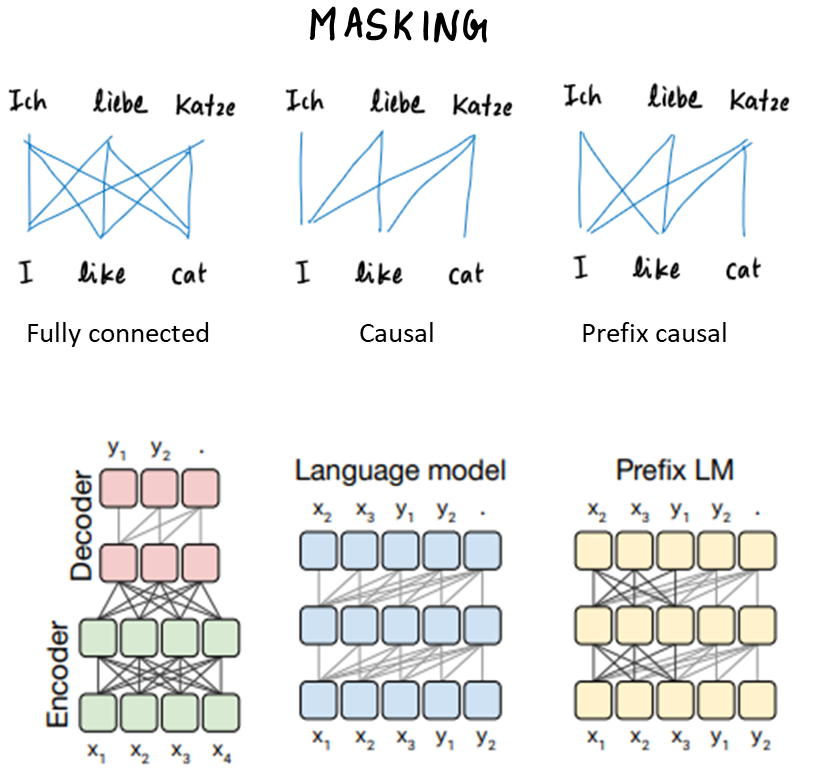
\includegraphics[width=0.7\textwidth]{images/masking.png}
\caption{Masking}
\label{fig:masking}
\end{figure} 

\subsection{Pre-training Objective}
In addition to the language modelling objective from the previous section, there are many other widely adopted strategies to train an unsupervised transfer learning model. \\
One of the most commonly used method is the de-noising objective where the some of the tokens in the input text is replaced by <M> tag. The objective of the model is to reconstruct the input sequence. It has many variants in itself. 

\begin{enumerate}
   


  \item The BERT style de-noising where the certain tokens are replaced by the <M> tag and some of them are replaced by random words \\ Input: Thank you <M> <M> me to your party apple week. \\Output: Thank you for inviting me to your party last week 
  \item MASS style is similar to BERT without the random word replacement \\ Input: Thank you <M> <M> me to your party last week.  \\ Output: Thank you for inviting me to your party last week  
  \item Deshuffling where the objective is to identify the correct order of the shuffled input tokens  \\ Input: party me for your to . last fun you inviting week Thank  \\  Output: Thank you for inviting me to your party last week.  
  \item Replacing spans of tokens instead of single token \\ Input: Thank you me to your party week   \\  Output: Thank you for inviting me to your party last week.
\end{enumerate}
Comparing a more detailed approach to corruption strategy, it is possible to adjust the corruption token length and corruption rate, in other words the number of tokens corrupted with respect to length of input sequence to monitor its impact on the performance measure. \\
Out of all the variants, BERT style pre-training objective that replaces 15 percent spans of length 3 achieves a better performance. 
\begin{figure}[H]
\centering
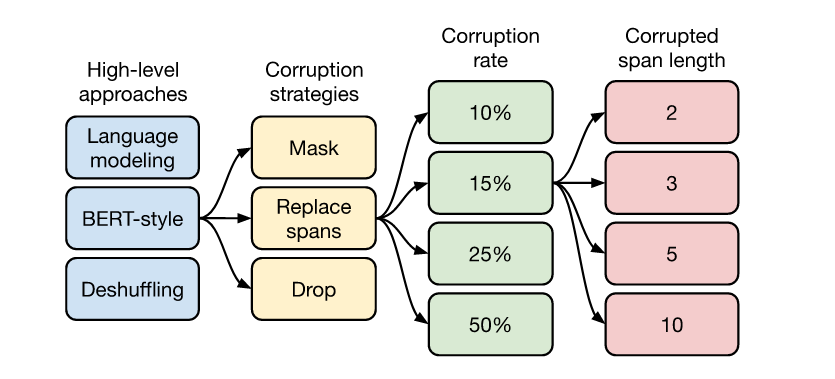
\includegraphics[width=0.7\textwidth]{images/preobj.png}
\caption{Pre-training objective}
\label{fig:preobj}
\end{figure} 

\subsection{Pre-training dataset}
Pre-training dataset is a very essential part of the transfer learning model. The quality and the type of the dataset might have a considerable effect on the performance of downstream and hence it is necessary to compare the different types of commonly used pre-training datasets. \\
Along with the C4 dataset previously discussed, the comparison was made on non-pre-processed C4 dataset, data extracted from Wikipedia, news dataset, data from content aggregation sites such as reddit, Wikipedia and book corpus. \\
The findings are presented in figure (right) below. It can be observed that Real news and Web text gives a better performance on glue tasks than the C4 dataset. Similarly, Wikipedia + TBC produces good performance on Super Glue task. The reason was identified as relatively high performance on MultiRC task of GLUE and Super GLUE which comes from a similar domain as the former dataset.  Thus, it can be argued that pre-training on in-domain unlabelled data can improve performance on downstream tasks. \\
In addition to dataset type, it is also beneficial to study the effect of repeating examples on performance of pre-training model. By repeating the data set 64, 256, 1,024, and 4,096 times during pre-training process, it is observed from the figure (left) below that the performance degrades as more and more examples are repeated during the training phase. 

\begin{figure}[H]
\centering
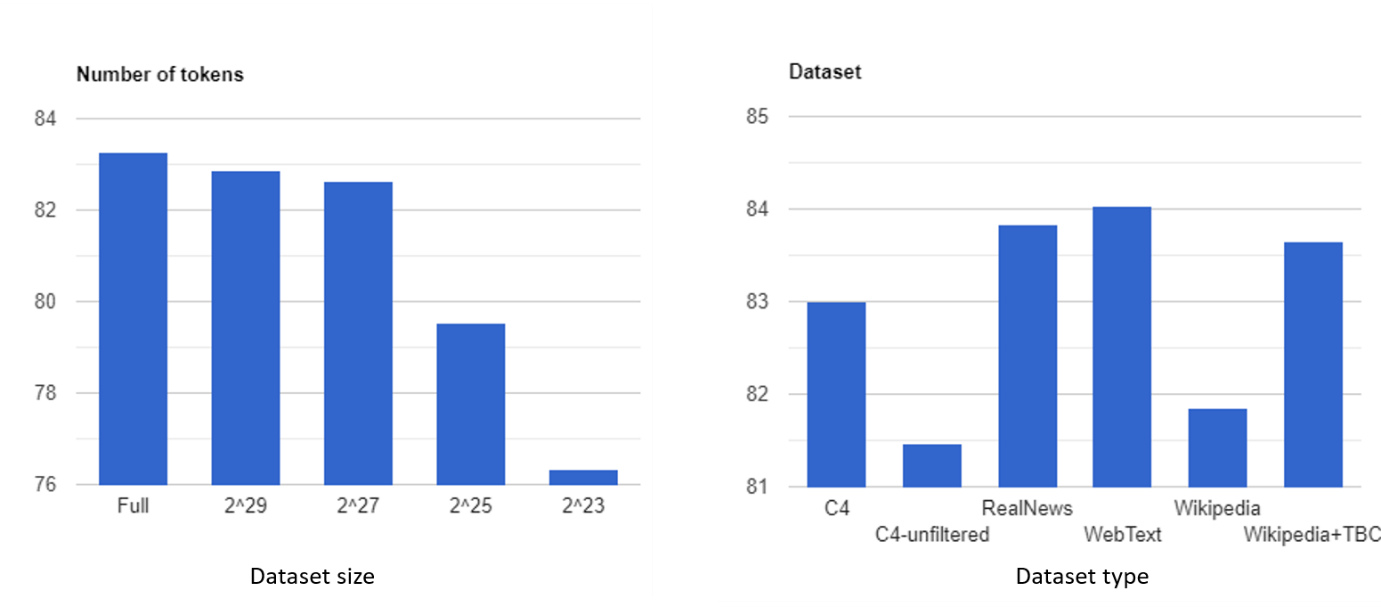
\includegraphics[width=0.7\textwidth]{images/predataset.png}
\caption{Pre-training Dataset}
\label{fig:predataset}
\end{figure}

\subsection{Downstream fine tuning}
Common approach to fine tuning on downstream is to fine tune only the last layers of the pre-trained model. This approach is usually seen in popular models such as BERT, XLNET. But in case of an encoder decoder architecture like T5 model, it is ideal to fine tune on all of the parameters of the model. But this computationally heavy and time consuming. \\
One of the alternate approaches considered here is the Adaptive layers approach. In this method, a dense ReLu block is added on top of each feedforward layer in the T5 model. This ReLu block has the same dimensionality d as the feed-forward layer and the parameters of the ReLu block alone is fine-tuned while training the model in the downstream task. It is observed that this method works well on low resource tasks such as SQUAD. \\
Another method is the Gradual unfreezing, where the parameters of the layers are fine tuned in a bottom up style. In other words, at first iteration the parameters of final layer are fine-tuned, in the second iteration last two layers are fine tuned and so on. Even though the performance of this method comparatively lower than fine tuning all of the parameters, it takes far less time than the latter approach. \\


\begin{figure}[H]
\centering
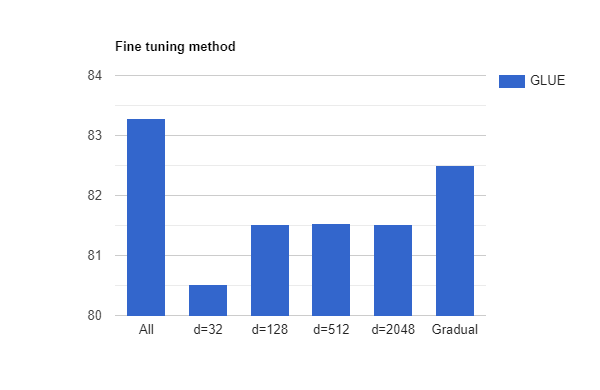
\includegraphics[width=0.7\textwidth]{images/finetune.png}
\caption{Downstream fine tuning}
\label{fig:finetune}
\end{figure}

\subsection{Multi task learning}
In order to incorporate the ability to perform multiple tasks simultaneously into the model, it is sufficient to mix training data from all of theses tasks since the T5 model is already defined as a text-to-text model. \\
Among the different methods, examples proportional method mixes data at the rate of  \\
\(r_{m} = min( e_{m},K)/ \sum min( e_{n},K)  \)
\\ Temperature scaled method is similar to the examples proportional method where the value of rm is raised to a power of T. The value of T limits how much the larger dataset is mixed. 
From the figure below it can be identified that for a specific value of K, the examples proportional methods works well and the temperature scaled method achieves even higher performance for a T value of 2. 

\begin{figure}[H]
\centering
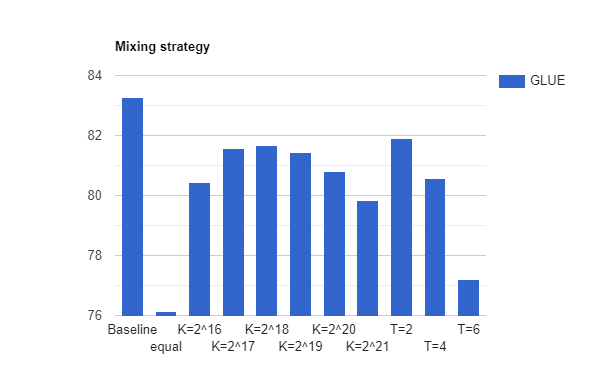
\includegraphics[width=0.9\textwidth]{images/multitask.png}
\caption{Multi task learning}
\label{fig:multitask}
\end{figure}

\subsection{Scaling}
It is very common in the transfer learning domain to improve the performance of the model significantly simply by scaling up the model in terms of model size S, training steps T or ensemble model E. 
With the assumption of 4 times more computational power, different scaling strategies are compared and it can be concluded that increasing both the model size and number of steps simultaneously achieves a significant increase in performance compared to other methods. 
The T5 large model is configured similar to BERT large model and consists of 4096 feedforward dimension, 16 attention head, 16/32 layers encoder-decoder block. The T5 3B model 16384 – feedforward layer dimension, 32 attention head and T5 11B model has 65538 – feedforward layer dimension, 128 attention head.